\chapter{The Photon in Quantum Electrodynamics (QED)}\index{Photon}\index{Quantum Electrodynamics (QED)}
\setcounter{section}{5}
\setcounter{subsection}{0}
\setcounter{subsubsection}{1}
\setcounter{secnumdepth}{3}
\setlength{\parindent}{0pt}
% Box styles
\tcbset{physikbox/.style={colback=blue!5!white, colframe=blue!75!black, fonttitle=\bfseries}}
\tcbset{mathebox/.style={colback=green!5!white, colframe=green!50!black, fonttitle=\bfseries}}
\tcbset{didaktikbox/.style={colback=yellow!5!white, colframe=yellow!50!black, fonttitle=\bfseries}}
\tcbset{hypobox/.style={colback=orange!5!white, colframe=orange!75!black, fonttitle=\bfseries}}
\tcbset{hinweisbox/.style={colback=gray!10!white, colframe=black!40!black, fonttitle=\bfseries}}
\tcbset{warnbox/.style={colback=red!10!white, colframe=red!40!black, fonttitle=\bfseries}}

\subsection{From the Photon to Quantum Electrodynamics}\index{Quantum Electrodynamics (QED)!Introduction}\index{Photoelectric Effect}\index{Compton Scattering}\index{Einstein, Albert}\index{Maxwell, James Clerk}\index{Exchange particle}
% Historical and theoretical transition: from classical electrodynamics via quantum optics to QED

The history of the photon begins with a paradox: Light, which since the 19th century was understood as an electromagnetic wave, showed behavior in certain experiments that could only be explained with a particle picture—particularly in the photoelectric effect and in Compton scattering.\index{Wave model}\index{Particle model}
These experiments led Einstein in 1905 to introduce the concept of the \emph{light quantum}.\index{Light quantum}
Although the photon model proved successful experimentally, it remained controversial for decades.\index{Photon model}

A complete theoretical understanding of light–matter interaction was achieved only with the development of \textbf{Quantum Electrodynamics} (QED).\index{Light–matter interaction}\index{Relativity!Special}\index{Quantum mechanics}
It unites Maxwell’s classical field theory with the principles of quantum mechanics and special relativity.
In QED, the photon is the exchange particle of the electromagnetic interaction—a massless, spin-1 gauge boson that can appear not only in real but also in virtual states.\index{Spin}\index{Masslessness}\index{Virtual photon}
(A compact introduction to the QED field formalism and the potential \(A^\mu\) can be found in Appendix~A, Section~\ref{anhangA:feldformalismus}.)
\newpage
\noindent
\vspace{1em}
\begin{tcolorbox}[physikbox, title=What is Quantum Electrodynamics?]
	\label{box:was ist quantenelektro}
	\small
	Quantum Electrodynamics describes how charged particles (e.g., electrons) exchange photons and thereby interact electromagnetically.\\
	The theory is based on quantized fields, Feynman diagrams, and a local gauge principle. It is the most precise physical theory ever tested experimentally.
\end{tcolorbox}
\vspace{1em}

The transition from classical to quantum field–theoretic understanding was anything but straightforward. At first, photons were treated as discrete packets of classical wave energy—a compromise between particle and wave pictures.\index{Quantum field theory}\index{Wave energy}
Only in the 1940s, through the work of Dirac, Feynman, Schwinger, and Tomonaga, did a consistent theory emerge that mathematically describes the photon as the quantum of the electromagnetic field.\index{Dirac, Paul A. M.}\index{Feynman, Richard P.}\index{Schwinger, Julian}\index{Tomonaga, Sin-Itiro}\index{Quantized field}

\textbf{What QED changes:}
\begin{itemize}
	\item Photons are no longer seen as light rays but as excitations of a quantized field.\index{Excitation (field)}\index{Light ray}
	\item Interaction occurs not continuously but in discrete processes (vertices).\index{Interaction!Vertex}
	\item Virtual photons—not directly observable but mathematically necessary—play a central role.\index{Virtual photon}
\end{itemize}
(For the transition from the classical field to quantization and to Feynman diagrams, see Appendix~A, Section~\ref{anhangA:feld_zu_qed}.)

This chapter introduces the properties of the photon within QED, beginning with its vector character, followed by its role as an exchange particle in Feynman diagrams, and ending with experimental confirmations of utmost precision.\index{Feynman diagram}

\subsection{The Vector Character of the Photon in QED}\index{Photon!Vector character}\index{Polarization!Transverse}\index{Spin}

The transverse polarization of the photon and its property as a spin-1 particle were already described in Section~3.6.\index{Helicity}
In Quantum Electrodynamics, however, this structure arises not only from experimental observation or classical equations, but from the underlying \emph{field formalism} and the \emph{gauge symmetry} of the theory.\index{Field formalism}\index{Gauge symmetry}
(A formal derivation of photon helicity is given in Appendix~A, Section~\ref{anhangA:helizitaet}; for polarization in Jones/Dirac notation, see \ref{anhangA:polarisation}.)

\vspace{1em}
\begin{tcolorbox}[physikbox, title=What is the Field Formalism?]
	\label{box:was ist Feldformalismus}
	\small
	In QED, photons are not “particles with trajectories,” but quantized excitations of a field: the electromagnetic potential \( A^\mu(x) \). Just as a water wave is a local displacement of the water surface, a photon is a discrete oscillation of the field—described simultaneously by quantum mechanics and relativity.
\end{tcolorbox}
\vspace{1em}
\index{Vector potential $A^\mu$}
(A short derivation of the Lorentz-covariant form of the four-potential \(A^\mu\) is given in Appendix~A, Section~\ref{anhangA:viererpotential}.)

The central mathematical starting point is the so-called \emph{Lagrangian density} \( \mathcal{L} \), from which the equations of motion of the field are derived.\index{Lagrangian density}\index{Equations of motion}
For the electromagnetic field it reads:

\[
\mathcal{L}_{\text{EM}} = -\frac{1}{4} F_{\mu\nu} F^{\mu\nu}
\quad \text{with} \quad F_{\mu\nu} = \partial_\mu A_\nu - \partial_\nu A_\mu
\]\index{Field strength tensor $F_{\mu\nu}$}
(Derivations of the field strength tensor and EM Lagrangian density: Appendix~A, Sections~\ref{anhangA:feldstaerketensor} and \ref{anhangA:lagrange_em}; for the energy–momentum relation see \ref{anhangA:energie_impuls}.)

This Lagrangian density leads—via the principle of least action—to Maxwell’s equations in their relativistic form.\index{Principle of least action}\index{Maxwell’s equations}
It is invariant under so-called \textbf{gauge transformations}:

\[
A^\mu(x) \rightarrow A^\mu(x) + \partial^\mu \Lambda(x)
\]\index{Gauge transformation}
(For local \(U(1)\) gauge symmetry, gauge fixing, and the Lorenz condition see Appendix~A, Section~\ref{anhangA:eichsymmetrie}.)
\vspace{1em}
\begin{tcolorbox}[physikbox, title=What Does Gauge Symmetry Mean?]
	\label{box:was bedeutet Eichsy}
	\small
	Gauge symmetry means that the electromagnetic potential \( A^\mu(x) \) can be changed locally without altering measurable quantities such as the electric field. This freedom is not just a mathematical trick but a structural principle: it determines which terms are allowed—and which are not.
\end{tcolorbox}

\textbf{Why is the photon massless?}\index{Masslessness}
A mass term of the form \( \frac{1}{2} m^2 A_\mu A^\mu \) would \emph{not} be invariant under this transformation. The requirement of gauge symmetry forbids it—the photon must be massless.\index{Mass term}\index{Gauge invariance}
(Formal argument via the Proca Lagrangian and broken gauge invariance: Appendix~A, Section~\ref{anhangA:masselosigkeit_proca}.)

\textbf{Why is the photon transverse?}\index{Transversality}
A vector field has four components, but not all are physically independent. Gauge freedom and Lorentz invariance allow the elimination of non-physical modes. In the end, only two permissible polarization states remain: the transverse ones with helicity \( +1 \) and \( -1 \).\index{Lorentz invariance}\index{Polarization states}
(Reduction of degrees of freedom, Lorenz condition, and trace/projector method: Appendix~A, Section~\ref{anhangA:transversalitaet}; see also \ref{anhangA:helizitaet}.)

\vspace{1em}
\begin{tcolorbox}[physikbox, title=Consequences of Gauge Symmetry]
	\label{box:folgen der Eichsy}
	\small
	The gauge symmetry of QED explains two fundamental properties of the photon:
	
	\begin{itemize}
		\item \textbf{Masslessness:} A mass term would not be gauge invariant—therefore the photon is necessarily massless.
		\item \textbf{Transversality:} The symmetry allows only two polarization modes—both perpendicular to the direction of propagation.
	\end{itemize}
\end{tcolorbox}

\textbf{Virtual photons—an exception}\index{Virtual photon}
While real photons possess only transverse states, so-called \emph{virtual photons}—appearing in the internal lines of Feynman diagrams—can also contain longitudinal or scalar components.\index{Longitudinal mode}\index{Scalar mode}
However, these are not observable and cancel completely in physical predictions (e.g., in the scattering amplitude).\index{Scattering amplitude}
(Longitudinal/scalar contributions in propagators and their cancellation in observables: Appendix~A, Section~\ref{anhangA:virtuelle_moden}.)

\textbf{Conclusion:}\index{Gauge symmetry!Consequences}
In QED, the structure of the photon does not result from extra assumptions but from the symmetric construction of the theory itself. Gauge symmetry replaces intuition—and creates order.

\subsection{Virtual Photons and Feynman Diagrams}\index{Virtual photon}\index{Feynman diagram}

\subsubsection{What Are Virtual Particles?}\index{Virtual particle}
\addcontentsline{toc}{subsubsection}{5.3.1 What Are Virtual Particles?}

Virtual particles—especially virtual photons—are central computational elements in quantum field theory.\index{Quantum field theory}
They differ fundamentally from real particles, which can be detected in a detector.\index{Real particle}\index{Detector}
Their existence is \textbf{mathematical in nature}—and yet their effects show up in real experiments.\index{Mathematical object}

\subsubsection*{Difference: Real or Virtual Particles}\index{On-shell}\index{Off-shell}
\phantomsection
\begin{table}[H]
	\centering
	\scriptsize 
	
	{\small
		\begin{center}
			\renewcommand{\arraystretch}{1.3}
			\begin{tabular}{|p{3cm}|p{3.0cm}|p{3.0cm}|}
				\hline
				\textbf{Property} & \textbf{Real Photons} & \textbf{Virtual Photons} \\
				\hline
				Observable in a detector & Yes (e.g., light quantum in the photoelectric effect) & No \\
				\hline
				Energy–momentum relation & $E = pc$ (on-shell) & $E^2 \ne p^2 c^2$ (off-shell) \\
				\hline
				Lifetime & Arbitrarily long (for stable particles) & Extremely short (due to uncertainty relation) \\
				\hline
				Physical existence & Yes & Only as a computational element in diagrams \\
				\hline
			\end{tabular}
		\end{center}
	}
\end{table}
\vspace{1em}

\begin{tcolorbox}[hinweisbox, title=On-Shell Condition]
	\label{box:On-shell-Bedingung}
	A particle is \textbf{on-shell} if it fulfills the relativistic energy–momentum relation:
	\[
	E^2 = p^2 c^2 + m^2 c^4
	\]
	For massless particles (e.g., photons) this reduces to:
	\[
	E = pc
	\]
	Off-shell states occur for virtual particles, which appear only in intermediate steps of calculations.
\end{tcolorbox}
\index{Energy–momentum relation}\index{Relativistic kinematics}

\subsubsection*{Time–Energy Uncertainty}\index{Uncertainty principle!Time–energy}
\phantomsection
According to Heisenberg’s uncertainty relation:
\[
\Delta E \cdot \Delta t \gtrsim \hbar
\]\index{Heisenberg, Werner}\index{$\hbar$}
For very short times $\Delta t$, it becomes possible to “violate” energy conservation temporarily—for example, by the appearance of a virtual photon with seemingly “wrong” energy.\index{Energy conservation}
This effect is not a rule violation but a consequence of quantum mechanics.\index{Quantum mechanics}

\subsubsection*{Interpretation}\index{Intermediate state}
\phantomsection

Virtual particles occur in \textbf{intermediate states}—for instance, when an electron briefly emits a photon that is immediately reabsorbed.\index{Electron}\index{Absorption}\index{Emission}
These processes are represented in \textbf{Feynman diagrams}. The virtual particles correspond to the \textbf{internal lines} of the diagram.\index{Internal lines (diagram)}

\vspace{1em}
\begin{tcolorbox}[physikbox, title=Virtual Particles in the Quantum Vacuum, label=box:virtuelle-teilchen]
	\label{box:virtuelle-teilchen}
	Virtual particles arise as intermediate states in quantum-mechanical interactions. They do not fulfill the classical energy–momentum relation (they are \emph{off-shell}) and cannot be observed directly.
	
	Nevertheless, their effects appear in the most precise experiments—for example, in the \textbf{Lamb shift} in the hydrogen spectrum or in the \textbf{anomaly of the electron’s $g$-factor}.
\end{tcolorbox}
\index{Quantum vacuum}\index{Lamb shift}\index{g-factor!Anomaly}\index{Hydrogen spectrum}

\vspace{1em}
\begin{tcolorbox}[hinweisbox, title=Indirect Evidence for Virtual Photons]
	\label{box:Nachweis virtueller Photonen}
	\small
	\begin{itemize}
		\item \textbf{Lamb shift:} In high-precision spectra of the hydrogen atom, a fine shift of the energy levels is observed, which can only be explained with quantum field–theoretic corrections—particularly the influence of virtual photons on the electron.
		\item \textbf{$g$-factor anomaly:} The electron possesses a magnetic moment that deviates slightly from the classical value $g = 2$. This deviation arises from loop processes in Feynman diagrams—with virtual photons as mediators.
	\end{itemize}
\end{tcolorbox}
\index{Loop processes}\index{Magnetic moment}\index{Electron}

\vspace{1em}
\begin{tcolorbox}[didaktikbox, title=Does Virtual Mean Less Real?, label=box:virtuell-denkfehler]
	\label{box:virtuell-denkfehler}
	The term “virtual” can easily be misleading. Virtual particles are \textbf{not simply “unreal” particles}—they are precisely defined mathematical objects in quantum field theory.\index{Quantum field theory}
	
	They follow their own rules and contribute decisively to the correct result—precisely because they \emph{do not} fulfill the conditions of real particles.
\end{tcolorbox}
\subsubsection*{Transition}\index{Coulomb force}\index{Scattering}
\phantomsection

In the next section, we consider how exactly these virtual photons mediate electromagnetic interaction in quantum field theory—from the classical Coulomb force to scattering processes.

\subsubsection{Virtual Photons as Exchange Particles}\index{Virtual photons!Exchange particle}\index{Exchange particle}\index{Interaction!Electromagnetic}

In classical physics, the electromagnetic force is described as a field produced by charges and acting on other charges—as in Coulomb’s law\index{Coulomb’s law} or in Maxwell’s equations.\index{Maxwell’s equations} In quantum field theory, by contrast, the force is mediated through the exchange of virtual photons.\index{Virtual photon}

These virtual photons appear in interaction processes between charged particles, without ever being observed as real light quanta.\index{Real photons} They are not detectable—yet they are the central element through which forces can be explained quantum mechanically.\index{Force!Quantum mediation}

\subsubsection*{Exchange Picture vs.\ Force Picture}\index{Exchange picture}\index{Force picture}\index{Momentum transfer}
\phantomsection

Instead of imagining a “force” in the classical sense, QED describes particles as sending each other \emph{virtual photons} that carry momentum. This creates the impression of an interaction.\index{QED}\index{Interaction!Exchange principle}

\vspace{1em}
\begin{tcolorbox}[physikbox, title=Virtual Photons as Force Mediators]
	\label{box:Virtuelle Photonen als kraftvermittler}
	Virtual photons transfer momentum between charged particles and thereby mediate the electromagnetic interaction. This process is the quantum field–theoretic explanation of forces such as the Coulomb force or magnetism.
	
	No real photon “flies” between the particles—the effect arises exclusively from mathematically described intermediate states in the Feynman diagram.
\end{tcolorbox}
\index{Force mediator}\index{Feynman diagrams}
\newpage
\noindent
\subsubsection*{Example: Electron–Electron Scattering}\index{Electron–electron scattering}\index{Møller scattering}\index{Scattering!Elastic}
\phantomsection
A particularly illustrative example is so-called \emph{Møller scattering}, in which two electrons scatter elastically. In classical physics, one would speak of a repulsive Coulomb force—in QED, however, the process is described as the exchange of a virtual photon between the electrons.\index{Coulomb force}\index{Virtual photon!Exchange}
\begin{figure}[H]
	\begin{center}
		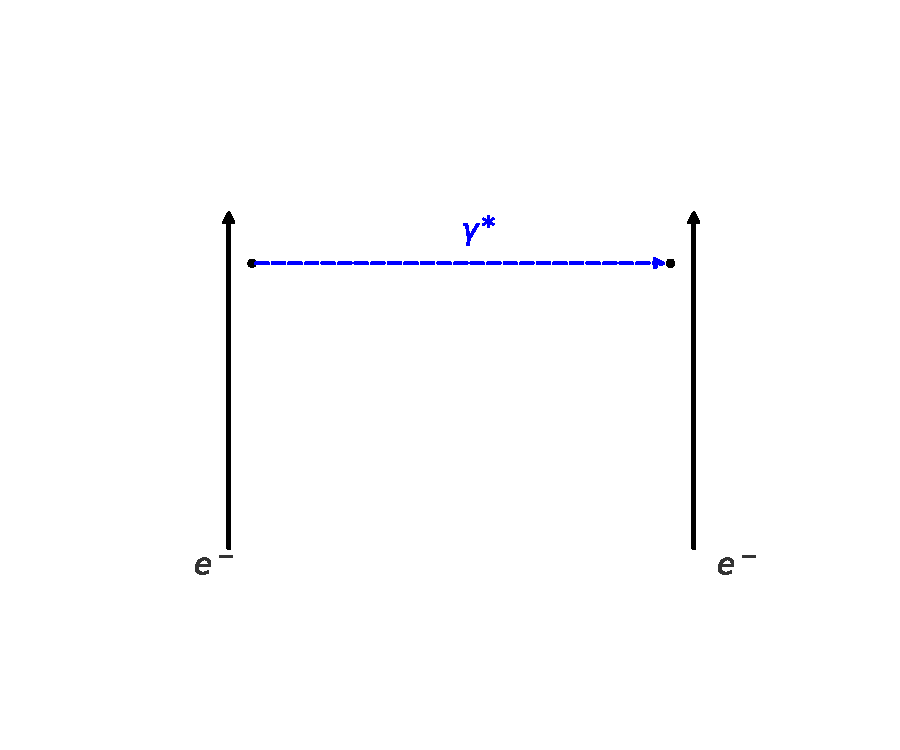
\includegraphics[width=0.4\textwidth]{bilder/moeller-diagramm.pdf}
	\end{center}
	\caption{The virtual photon is shown here as the internal line of the Feynman diagram. It transfers momentum—although it never exists as a real particle.}
\end{figure}

\subsubsection*{What Does This Diagram Show?}\index{Feynman diagrams!Interpretation}\index{Internal lines (diagrams)}\index{Vertex}\index{Momentum transfer}\index{Energy transfer}
\phantomsection
The Feynman diagram represents a typical \textbf{Møller scattering}—the elastic scattering of two electrons via the exchange of a virtual photon. The time axis runs from bottom to top.\index{Time axis (diagram)}

\begin{itemize}
	\item \textbf{Two electrons} enter the diagram from below (left and right sides). They approach each other and interact.\index{Electron}
	
	\item The \textbf{virtual photon} (depicted by the dashed blue line and the symbol $\gamma^*$) is exchanged between the electrons.\index{Photon!Virtual $\gamma^*$} It is \emph{not real}, but an intermediate state in the quantum field–theoretic calculation.\index{Intermediate state}
	
	\item The photon transfers momentum and energy—causing the electrons to change direction and leave the interaction region scattered upward.\index{Scattering angle}
	
	\item The two \textbf{vertices} (connection points) show where the interaction is localized. Mathematically, the momentum transfer takes place at these points.\index{Vertex}
\end{itemize}

\begin{tcolorbox}[didaktikbox, title=What Does the Feynman Diagram Really Show?]
	\label{box:Was zeigt das Feynman-Diagramm wirklich}
	The Møller scattering diagram does not show a real photon “flying” between electrons. Rather, it describes a quantum-mechanical intermediate state:
	
	A \textbf{virtual photon} mediates the interaction—mathematically within perturbation theory. This photon does not satisfy the classical relation $E = pc$, it exists only as an \emph{off-shell} intermediate state and transfers momentum.
	
	Real effects such as scattering angles and energy distributions can be calculated from it—without a photon ever being detected.
\end{tcolorbox}
\index{Perturbation theory}\index{Off-shell}\index{Energy distribution}

\subsubsection*{No Direct Observability—but Measurable Effect}\index{Cross section}\index{Observables}
\phantomsection
Virtual photons cannot be detected. Yet they influence measurable quantities: cross sections, scattering angles, and energy distributions can be described with high accuracy through the underlying exchange mechanism.

\subsubsection*{Distinction from Real Photon Production}\index{Compton effect}\index{Photon processes}\index{Exchange diagrams}\index{Real photons}
\phantomsection
An important difference: In the \emph{Compton effect}, a \textbf{real} photon is scattered—with detection in the experiment. In \textbf{virtual exchange}, by contrast, no photon participates as a real particle. This is the fundamental distinction between \textbf{exchange diagrams} and \textbf{photon processes}.

\vspace{1em}
\begin{tcolorbox}[didaktikbox, title=No Need for an “Invisible Force”]
	\label{box:unsichtbare Kraft}
	In quantum field theory, there is no longer a need for a classical force field acting between two charges. Instead, interactions arise through the exchange of virtual particles—in this case, virtual photons.
	
	The classical picture of action at a distance is replaced by a local, quantized exchange principle.
\end{tcolorbox}
\index{Action at a distance}\index{Locality}\index{Exchange principle}
\newpage
\noindent
\subsubsection{Feynman Diagrams as Visual Aids for Calculation}\index{Feynman diagrams!Computational aid}\index{Probability amplitude}\index{Perturbation theory}

The so-called \textbf{Feynman diagrams} are a central tool of quantum field theory—especially in Quantum Electrodynamics (QED).\index{Quantum field theory}\index{QED} They serve as a \emph{graphical notation} for mathematical terms in perturbation theory and help structure complex processes in an illustrative way.

A diagram does not represent a real “sequence in space and time,” but encodes a probability amplitude. Nevertheless, measurable physical quantities such as scattering angles, cross sections, or lifetimes can be calculated from it.\index{Lifetime}

\subsubsection*{Elements of a Feynman Diagram}\index{Fermion lines}\index{Photon lines}\index{Vertices}\index{Time axis (diagram)}
\phantomsection
\begin{itemize}
	\item \textbf{Fermion lines:} solid lines with arrows—e.g., electrons or positrons
	\item \textbf{Photon lines:} wavy or dashed lines—depending on convention
	\item \textbf{Vertices:} points where particles “interact,” i.e., momentum is transferred
	\item \textbf{Time axis:} usually bottom to top, or left to right
\end{itemize}
\begin{figure}[H]
	\begin{center}
		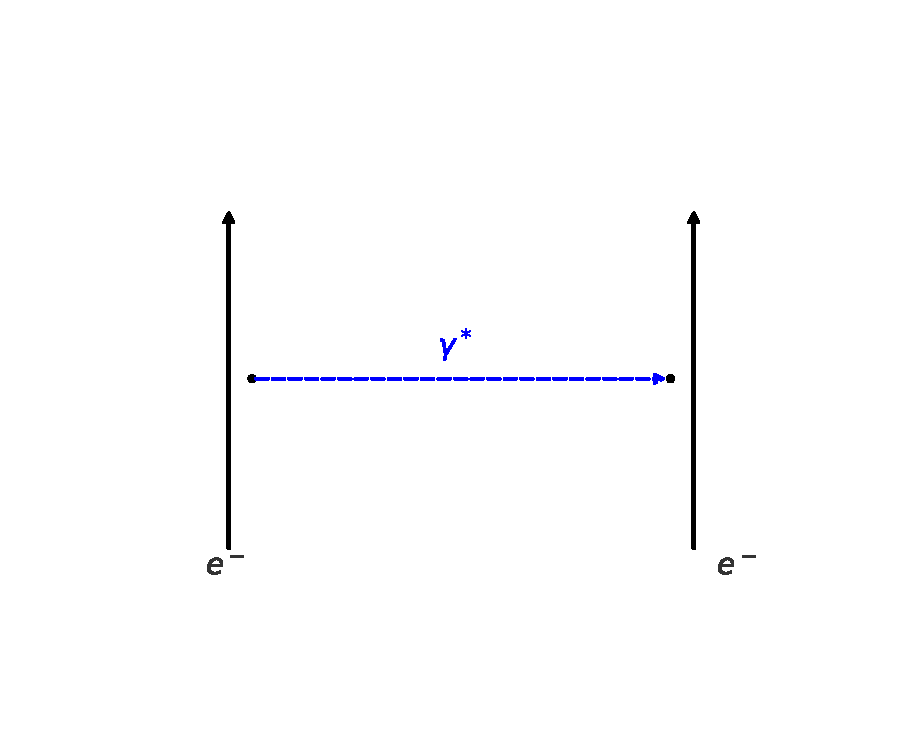
\includegraphics[width=0.45\textwidth]{bilder/feynman-einphoton.pdf}
	\end{center}
	\caption{Feynman diagram}
\end{figure}
\newpage
\noindent
\vspace{0.5em}
\begin{tcolorbox}[physikbox, title=What a Feynman Diagram Really Shows]
	\label{box:Was ein Feynman-Diagramm}
	A Feynman diagram is not a classical motion picture, but a symbolic representation of a mathematical integral over all possible paths of a process. It encodes the structure of the probability amplitude, not the exact trajectory of individual particles.
\end{tcolorbox}
\index{Path integral}

\subsubsection*{Example: Single-Photon Exchange}\index{Single-photon exchange}\index{Electron–electron scattering}\index{Momentum transfer}
\phantomsection
In elastic electron–electron scattering, the corresponding Feynman diagram consists of two incoming and two outgoing electron lines, plus one virtual photon line in between. This diagram symbolically represents a formula summing over all possible momentum transfers and times—it does not replace reality but reflects it probabilistically.\index{Probabilistic description}

\subsubsection*{More than Just Pictures—Diagram Rules}
\phantomsection
\index{Feynman rules}\index{Propagator}\index{Coupling constant}\index{Charge!Electric}\index{Amplitude!Scattering amplitude}
Every Feynman diagram corresponds to a mathematical expression. The so-called \emph{Feynman rules} assign, for example, a fraction term (propagator) to each line, a coupling constant (e.g., $e$) to each vertex, and an integral over momenta to the whole diagram. The sum of all possible diagrams up to a certain order yields the physically measurable quantity.\index{Momentum-space integral}\index{Order (perturbation theory)}

\vspace{1em}
\begin{tcolorbox}[didaktikbox, title=A Diagram Is Not Reality]
	\label{boxx:Diagramm ist nicht gleich realität}
	A common misunderstanding is that a Feynman diagram shows a real process—for example, a photon “flying.” In fact, it describes a \emph{superposition of all possible intermediate states}, summarized in a quantum-mechanical amplitude. It is therefore a computational tool, not a film of what happens.
\end{tcolorbox}
\index{Superposition}\index{Intermediate state}

\subsubsection{Illustrative Diagrams}\index{Processes!QED}\index{Virtual photons!vs.\ real photons}\index{Real photons}
\phantomsection

To better understand the role of virtual photons compared with real photons, it is worth looking at typical processes in Quantum Electrodynamics. Feynman diagrams clearly indicate whether a photon is real (detectable) or only virtual (mediating interaction).

\subsubsection*{1. Virtual Exchange: Møller Scattering (Elastic $e^-e^-$ Collision)}\index{Møller scattering}\index{Scattering!Elastic}\index{Virtual photons!Exchange}
\phantomsection
In this process, two electrons scatter elastically through the exchange of a virtual photon. The photon is not real—it only transfers momentum.\index{Momentum transfer}
\begin{figure}[H]
	\begin{center}
		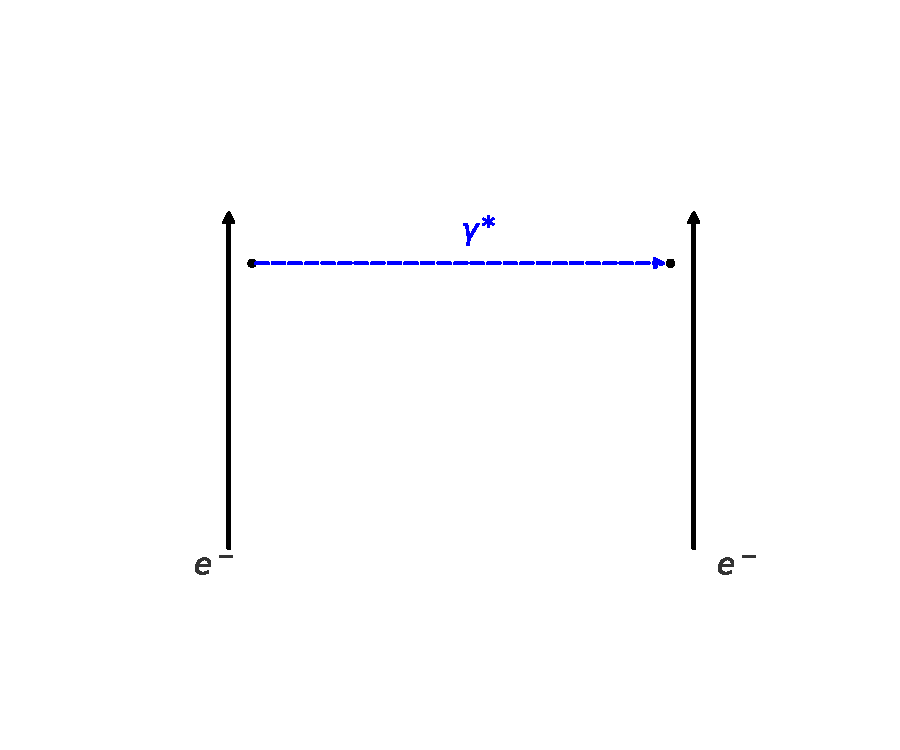
\includegraphics[width=0.42\textwidth]{bilder/moeller-diagramm.pdf}
	\end{center}
	\caption{Virtual photon}
\end{figure}

\begin{tcolorbox}[physikbox, title=Virtual Photon]
	\label{box:virtuelles Photon}
	The exchanged photon is virtual—it does not exist as a real particle. It transfers momentum and energy but does not fulfill $E = pc$.
\end{tcolorbox}
\index{Photon!Virtual}\index{Energy transfer}
\newpage
\noindent
\subsubsection*{2. Real Photon: Compton Scattering}\index{Compton effect}\index{Real photons}\index{Feynman diagrams!Compton scattering}\index{On-shell}\index{Electron propagator}\index{Vertex}
\phantomsection
In the Compton effect, a \textbf{real} photon is scattered by an electron. Both the incoming and outgoing photons are real, detectable particles.\index{Detection} The Feynman diagram shows two vertices with an internal electron propagator.\index{Propagator!Electron}\index{Vertices}

\begin{figure}[H]
	\begin{center}
		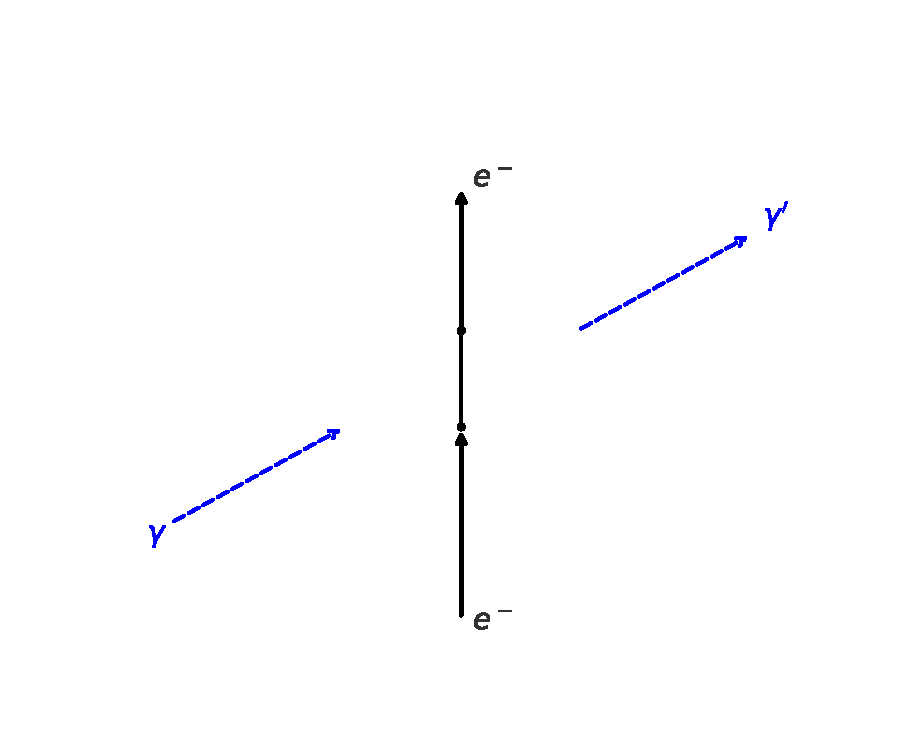
\includegraphics[width=0.5\textwidth]{bilder/compton-diagramm.pdf}
	\end{center}
	\caption{Real photon}
\end{figure}

\begin{tcolorbox}[physikbox, title=Real Photons]
	\label{box:Reale Photonen}
	In Compton scattering, photons appear as real particles. They are measurable and fulfill the on-shell condition $E = pc$.
\end{tcolorbox}
\index{Photon!Real}\index{On-shell condition}
\newpage
\noindent
\subsubsection*{3. Loop Diagrams: Self-Interaction and $g$-Factor}\index{Loop diagrams}\index{Self-energy}\index{Vertex correction}\index{g-factor!Anomaly}
\phantomsection
In higher orders of perturbation theory, closed loops appear in Feynman diagrams—for example, when an electron interacts with itself via a virtual photon.\index{Virtual photon} Such diagrams explain, among other things, the anomaly of the $g$-factor.\index{Anomaly!$g$-factor}
\begin{figure}[H]
	\begin{center}
		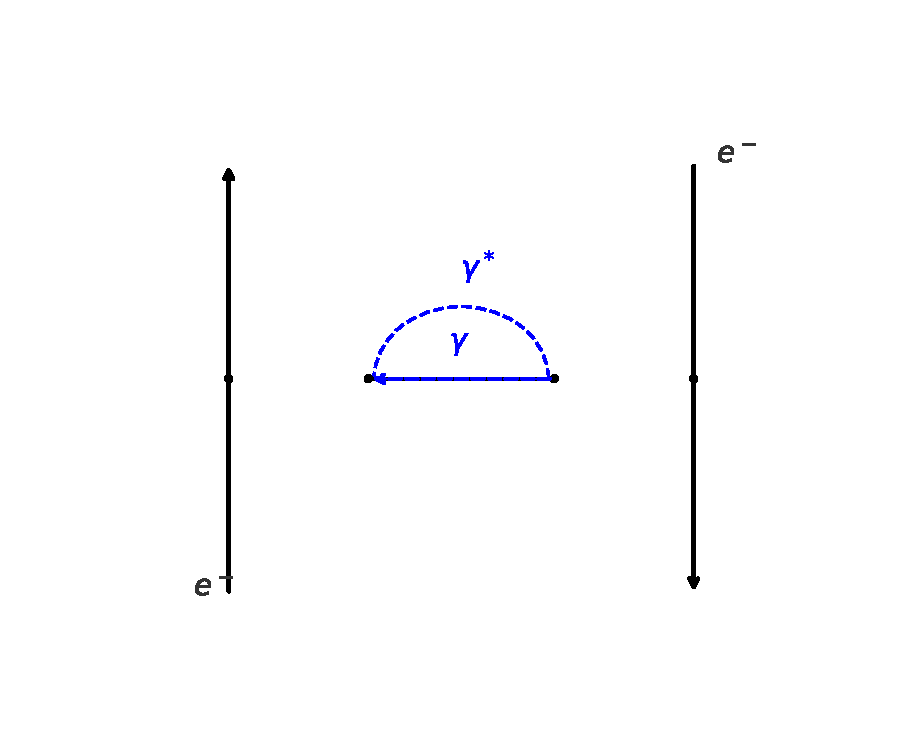
\includegraphics[width=0.4\textwidth]{bilder/vertex-korrektur.pdf}
	\end{center}
	\caption{Loop diagram}
\end{figure}

\begin{tcolorbox}[hinweisbox, title=Loop Diagrams and Precision Effects]
	\label{box:Schleifendiagramme}
	Loops with virtual photons provide corrections to simple processes—for example, for the exact value of the electron $g$-factor or the Lamb shift. These effects have been confirmed experimentally with high precision.
\end{tcolorbox}
\index{Lamb shift}\index{Precision experiments}

\subsubsection*{Didactic Comparison}\index{Didactic comparison}\index{Photons!Real vs.\ virtual}
\phantomsection
\begin{itemize}
	\item \textbf{Virtual photons} appear as internal lines in diagrams. They are not directly observable but are physically effective.\index{Internal lines}\index{Detection!Indirect}
	\item \textbf{Real photons} are external lines. They can be measured and are on-shell.\index{External lines}
\end{itemize}

\begin{tcolorbox}[didaktikbox, title=Real or Virtual Photons in the Diagram]
	\label{box:Reale oder virtuelle Photonen}
	Whether a photon is real or virtual is seen from whether it is shown as an incoming or outgoing particle. Only real photons are observable. Virtual photons are internal lines—they “exist” only within the calculation.
\end{tcolorbox}

\index{Observability}\index{Incoming particles}\index{Outgoing particles}
\newpage
\noindent
\subsubsection{Significance for QED}\index{QED!Significance}\index{Electromagnetic interaction}

Quantum Electrodynamics (QED) is the most precisely confirmed theory in physics. Its enormous accuracy would be unthinkable without the concept of virtual photons and Feynman diagrams.\index{Feynman diagrams}\index{Virtual photons}
\subsubsection*{Central Role of Virtual Photons}\index{Virtual photons!Central role}\index{Perturbation theory}
\phantomsection
Virtual photons enable the calculation of electromagnetic interaction between charged particles on the quantum level. They appear in all orders of perturbation theory—from simple exchange processes to complex loop corrections.\index{Exchange processes}\index{Loop corrections}

\vspace{1em}
\begin{tcolorbox}[physikbox, title=No QED Without Virtual Photons]
	\label{box:Ohne virtuelle Photonen keine}
	Virtual photons are the foundation of the quantum field–theoretic description of electromagnetic processes. Without them, QED could neither mediate forces nor make quantitative predictions.
\end{tcolorbox}

\subsubsection*{Feynman Diagrams as Methodological Backbone}\index{Feynman diagrams!Method}\index{Amplitudes!Probability}
\phantomsection
Feynman diagrams provide not only an illustrative representation but also a precise computational prescription. For every possible interaction, all allowed diagrams can be drawn and translated into a mathematical expression. The sum of all diagrams yields the observable amplitude.\index{Sum over diagrams}

\subsubsection*{Example: Calculation of the $g$-Factor}\index{g-factor!Electron}\index{Anomalous magnetic moment}
\phantomsection
The deviation of the electron’s gyromagnetic factor from the classical value $g = 2$ is one of the most accurate experiments in modern physics. The correction arises from a loop process with a virtual photon—that is, from a second-order Feynman diagram.\index{Second order}

\subsubsection*{Accuracy of the Theory}\index{QED!Accuracy}\index{Theory–experiment comparison}
\phantomsection
The theoretically calculated values for quantities such as the Lamb shift, the electron $g$-factor, or scattering angles in electron collisions agree with measurements to many decimal places.\index{Scattering angle}\index{Electron scattering}

\vspace{1em}
\begin{tcolorbox}[didaktikbox, title=Quantum Electrodynamics as a Success Story]
	\label{box:Die Quantenelekrodynamik}
	QED is not only an elegant theory—it delivers, with the help of virtual particles and Feynman diagrams, quantitative predictions with an accuracy of up to 12 decimal places. The role of the photon—even as a virtual particle—is central.
\end{tcolorbox}
\index{Success story}\index{Accuracy!12 decimal places}

\subsubsection{Limits and Misconceptions}\index{Limits of QED}\index{Misconceptions!Feynman diagrams}

Despite their illustrative representation, Feynman diagrams must not be misunderstood as pictorial descriptions of real processes. Virtual photons do not exist in the classical sense—they are mathematical objects within an approximation method.\index{Approximation method}

\subsubsection*{Virtual Photons Do Not Fly}\index{Virtual photons!Do not fly}\index{Particle trajectory!Not classical}
\phantomsection
It is misleading to say that a virtual photon “flies back and forth between two electrons.” Virtual particles are not measurable, not localized, and do not satisfy a classical equation of motion. Their role consists exclusively in mediating interaction within a quantum-mechanical computational model.\index{Localization}\index{Equation of motion!Classical}

\vspace{0.5em}
\begin{tcolorbox}[didaktikbox, title=No Particle Trajectory in the Diagram]
	\label{box: Keine Teilchenbahn im Diagramm}
	A Feynman diagram does not describe motion in space or a classical flight path. It represents a symbolic structure for calculating an amplitude. The “lines” in the diagram are not trajectories but terms in a formula.
\end{tcolorbox}
\index{Lines!Not trajectories}

\subsubsection*{Off-Shell Means: No Energy–Momentum Relation}\index{Off-shell}\index{Energy–momentum relation}
\phantomsection
Virtual photons do not satisfy the familiar relation $E = pc$. They are \emph{off-shell}, i.e., they temporarily violate the energy–momentum balance—within the framework of Heisenberg’s uncertainty relation.\index{Uncertainty principle!Time–energy} This is not a weakness of the theory but one of its central features.

\subsubsection*{Diagrams Are Not Exact Pictures}\index{Feynman diagrams!Not pictures}\index{Reality!vs.\ Model}
\phantomsection
Another misconception is to assume that Feynman diagrams show “what really happens.” In fact, they contain no statement about the sequence of events, real locations, or classical times. The diagrams represent probability amplitudes—not observations.\index{Observations}

\vspace{0.5em}
\begin{tcolorbox}[warnbox, title=Warning: Do Not Take Feynman Diagrams Literally!]
	\label{box:Warnung}
	Feynman diagrams are a powerful computational tool—but not sketches of reality. Interpreting them as “sequences of particle flights” misses the essence of quantum field theory.
\end{tcolorbox}
\index{Warning}

\subsubsection*{Limits of Validity}\index{Range of validity}\index{Strong interaction!Limits of perturbation theory}\index{Lattice gauge theory}
\phantomsection
QED—and with it the concept of virtual photons—is a perturbation theory. It works excellently for small coupling constants (e.g., in electrodynamics), but fails for strong interactions. There, other methods (e.g., lattice theory) are required.

\subsubsection*{Conclusion of This Section}\index{Conclusion!Virtual photons and diagrams}
\phantomsection
Virtual photons and Feynman diagrams are central concepts in QED—but they must be interpreted correctly: not as “flying particles” but as building blocks of a mathematical theory with enormous predictive power.

\subsubsection{Summary}\index{Summary!QED interpretation}

Virtual photons do not appear in detectors—but they determine what is measured there. They are the invisible carriers of electromagnetic interaction in the quantum world. Feynman diagrams help capture their effect mathematically, without attributing to them a classical reality.

QED would not be possible without these concepts—and it is precisely these seemingly abstract building blocks that make it the most precise theory in physics.\index{Most precise theory}

\subsection{The QED Formalism}\index{QED!Formalism}\index{Lagrangian density!QED}\index{Gauge invariance}\index{Renormalization@Renormalization (general)}
% Coupling constant, gauge invariance, renormalization, propagators

Quantum Electrodynamics—QED for short—is the field theory of the electromagnetic interaction.\index{Field theory} It describes how electrons, positrons, and photons behave quantum mechanically and interact with each other.\index{Electron}\index{Positron}\index{Photon}

In the previous chapter we saw how Feynman diagrams are used to represent processes such as electron scattering, the Compton effect, or self-interactions.\index{Electron scattering}\index{Compton effect}\index{Self-interaction} But these diagrams are not a substitute for the underlying theory—they are \emph{derived tools}.\index{Tools!Derived}

In this chapter, we go one step deeper: we look at the \textbf{mathematical structure} of QED.\index{Mathematical structure} At the center is the so-called \textbf{Lagrangian density}, from which all predictions of the theory can be derived—from the structure of the interaction to the Feynman rules.\index{Feynman rules}

It turns out: The whole of Quantum Electrodynamics can be built from just a few principles—especially the requirement of \textbf{gauge invariance} and of \textbf{relativity}.\index{Relativity} These principles determine not only the form of the equations but also how the photon fits into the theory as a massless interaction particle.\index{Photon!Massless}\index{Interaction particle}

The goal of this chapter is therefore to understand QED from its foundations—not as a collection of computational rules, but as an elegantly structured theory with enormous predictive power.\index{Predictive power}

\vspace{1em}
\begin{tcolorbox}[hinweisbox, title=Note for Readers]
	\label{box:Hinweis füe Leser}
	This chapter introduces the mathematical structure of Quantum Electrodynamics (QED). It is aimed at readers interested in the theoretical derivation of photon interaction. 
	
	Readers primarily interested in experimental confirmation and applications may skip directly to Chapter~5.5—without losing the main thread of the book.
\end{tcolorbox}


\subsubsection{Basic Idea of QED as a Field Theory}\index{Basic idea!QED}\index{Field theory!Basics}

Quantum Electrodynamics is a \textbf{field theory}.\index{Field theory} This means: it does not describe individual particles but fields that propagate through space and interact with each other.

An electron is not treated as a point particle but as an excitation of a \emph{Dirac field}.\index{Dirac field} Light—or more precisely: the photon—is likewise neither a wave nor a classical particle, but the excitation of an \emph{electromagnetic field}, which itself is quantized.\index{Electromagnetic field!Quantized}

\subsubsection*{Particles as Fields}\index{Particles as fields}\index{Fock space}\index{Excitations}
\phantomsection
Instead of describing the exchange of particles, QED works with fields such as:
\begin{itemize}
	\item \textbf{Electron field} $\psi(x)$ (Dirac field)\index{Electron field $\psi$}
	\item \textbf{Photon field} $A^\mu(x)$ (Four-potential)\index{Photon field $A^\mu$}\index{Four-potential}
\end{itemize}

The state of an electron (e.g., position, momentum, spin) is described by a wave function within the Dirac field.\index{Wave function}\index{Spin} A photon, on the other hand, is an excitation of the quantized field $A^\mu$—more precisely: a \textbf{Fock state} with one photon.\index{Fock state}

\subsubsection*{Interaction Through Coupling of Fields}\index{Interaction!Field coupling}
\phantomsection
The central idea of QED is that these two fields are \emph{coupled} to each other. The interaction does not take place directly between particles, but through terms in the so-called \textbf{Lagrangian density}:\index{Lagrangian density}
\[
\mathcal{L}_{\text{int}} = -e \, \bar{\psi} \gamma^\mu \psi \, A_\mu
\]
\index{Coupling term $-e\bar\psi\gamma^\mu\psi A_\mu$}

This expression describes that the electron field $\psi$ couples to the electromagnetic field $A_\mu$—in other words, it “feels” the presence of a photon.\index{Coupling!Electron–photon} The coupling term contains exactly the structure that later appears in Feynman diagrams as a vertex.\index{Vertex}

\vspace{0.5em}
\begin{tcolorbox}[physikbox, title=Field Theory Instead of Particle Mechanics]
	\label{box:Feldtheorie statt Teilchenmechanik}
	In QED, electrons and photons are not treated as classical particles but as quantized fields. Their interaction arises from a coupling term in the Lagrangian density—not from a classical force.
\end{tcolorbox}
\index{Particle mechanics!vs.\ Field theory}

\subsubsection*{Why This Approach Is Necessary}\index{Motivation!QED}\index{Limits!Classical electrodynamics}
\phantomsection
Classical electrodynamics (Maxwell’s equations) cannot explain many phenomena:\index{Maxwell’s equations}
\begin{itemize}
	\item No quantized energy transfer\index{Energy transfer!Quantized}
	\item No concept of the photon\index{Photon!Concept}
	\item No way to describe scattering at the quantum level\index{Scattering!Quantum level}
\end{itemize}

Only a quantized field theory makes it possible to describe processes such as the photoelectric effect, Compton scattering, or electron–positron annihilation correctly.\index{Photoelectric effect}\index{Compton effect}\index{Annihilation!Electron–positron}
\newpage
\noindent
\vspace{0.5em}
\begin{tcolorbox}[didaktikbox, title=Why Not Simply Classical?]
	\label{box:Warum nicht einfach klassisch?}
	Quantum field theory extends quantum mechanics to systems with variable particle number. Only in this way can creation and annihilation of photons or electrons be described rigorously. Without this approach, one could not derive Feynman diagrams—nor achieve the precision results of QED.
\end{tcolorbox}
\index{Quantum field theory}\index{Quantum mechanics}\index{Creation and annihilation}

\subsubsection{The QED Lagrangian Density}\index{Lagrangian density!QED}

At the heart of QED is the so-called \textbf{Lagrangian density}, from which all equations of the theory can be derived. It contains both the free fields (electron, photon) and their interaction.

The full QED Lagrangian density reads:
\[
\mathcal{L}_{\text{QED}} = \bar{\psi}(i \gamma^\mu \partial_\mu - m)\psi - \frac{1}{4}F_{\mu\nu}F^{\mu\nu} - e \bar{\psi} \gamma^\mu \psi A_\mu
\]

\begin{tcolorbox}[mathebox, title=Structure of the QED Lagrangian Density]
	\label{box:Sufbau der QED-Langrangedichte}
	\begin{itemize}
		\item $\bar{\psi}(i \gamma^\mu \partial_\mu - m)\psi$: Dirac term for the free electron field\index{Dirac term}
		\item $-\frac{1}{4}F_{\mu\nu}F^{\mu\nu}$: Kinetic term for the photon (Maxwell part)\index{Maxwell term}\index{Kinetic term}
		\item $-e \bar{\psi} \gamma^\mu \psi A_\mu$: Coupling between electron field and electromagnetic field\index{Coupling!Electron–photon}
	\end{itemize}
\end{tcolorbox}

\subsubsection*{Meaning of the Terms}\index{Interpretation of terms}\index{Free field}
\phantomsection
Each part of the Lagrangian density corresponds to a component of the theory:

- The first term describes the \textbf{free Dirac field}—that is, an electron or positron without external influence.\index{Free Dirac field}
- The second term is the \textbf{free electromagnetic field strength}—the quantum version of the Maxwell field.\index{Free photon field}
- The third term describes the \textbf{interaction} between electron and photon—the core of QED.\index{Interaction!Electron–photon}

\subsubsection*{Field Strength Tensor}\index{Field strength tensor $F_{\mu\nu}$}
\phantomsection
The expression $F_{\mu\nu}$ is the so-called \textbf{field strength tensor}, defined as:
\[
F_{\mu\nu} = \partial_\mu A_\nu - \partial_\nu A_\mu
\]
\index{Lorentz invariance}

It contains both the electric and the magnetic field—packaged into a single relativistic object. The term $F_{\mu\nu}F^{\mu\nu}$ is invariant under Lorentz transformations.

\vspace{1em}
\begin{tcolorbox}[physikbox, title=Photon Field from the Lagrangian Density]
	\label{box:Photonenfeld aus der Lagrangedichte}
	The photon’s quantum nature arises in QED from the quantization of the field $A^\mu$ within the Maxwell structure. The field strength tensor $F_{\mu\nu}$ contains the dynamics of the photon as a quantized gauge field.
\end{tcolorbox}
\index{Gauge field}

\subsubsection*{Interaction as Coupling Terms}\index{Interaction!Coupling terms}\index{QED vertex}
\phantomsection
The interaction term\\$-e \bar{\psi} \gamma^\mu \psi A_\mu$ describes the coupling of electrons to the photon. 

From this term follows directly the structure of the QED vertex in Feynman diagrams:
\begin{figure}[H]
	
	\[
	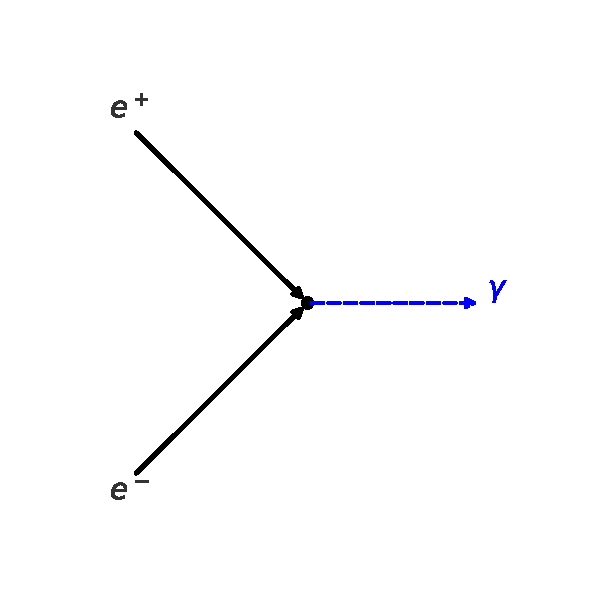
\includegraphics[height=8.5em]{bilder/qed-vertex.pdf} \quad \Rightarrow \quad -ie\gamma^\mu
	\]
	\caption{Interaction term}
\end{figure}
\vspace{0.5em}
\begin{tcolorbox}[didaktikbox, title=From Lagrangian Term to Feynman Vertex]
	\label{box:Vom Lagrange-Term zum Feynmann-Vertax}
	The coupling in the Lagrangian density generates the QED vertex: one electron, one positron, one photon meet at a point. This structure forms the basis of all diagrams in QED.
\end{tcolorbox}
\index{Vertex factor $-ie\gamma^\mu$}
\subsubsection*{Gauge Invariance as a Principle}\index{Gauge invariance!Local}\index{Gauge transformation}
\phantomsection
The form of the QED Lagrangian density is not chosen arbitrarily. It results from the requirement that the theory be \textbf{locally gauge invariant}—that is, symmetric under transformations of the form:
\[
\psi(x) \rightarrow e^{i\alpha(x)} \psi(x), \qquad A_\mu(x) \rightarrow A_\mu(x) - \frac{1}{e} \partial_\mu \alpha(x)
\]

Only with this structure does the theory remain consistent, relativistically invariant, and quantizable.\index{Quantizability}

\subsubsection{Coupling Between Electrons and Photons}\index{Coupling!Electron–photon}\index{Local gauge invariance}

In QED, the interaction between electron and photon does not arise “from the outside,” but follows from a fundamental principle: \textbf{local gauge invariance}. This symmetry forces us to introduce the photon as the coupling partner of the electron field.

\subsubsection*{Global and Local Phase Transformations}\index{Phase transformation!Global}\index{Phase transformation!Local}
\phantomsection
A Dirac field $\psi$ is invariant under a \textbf{global} phase transformation:
\[
\psi(x) \rightarrow e^{i\alpha} \psi(x)
\]
The Lagrangian density remains unchanged—this is a symmetry.

If, however, one demands that $\alpha$ depends on position, i.e.
\[
\psi(x) \rightarrow e^{i\alpha(x)} \psi(x)
\]
one speaks of a \textbf{local gauge transformation}. This destroys the invariance of the Lagrangian density—unless one introduces an additional field $A_\mu(x)$ that co-transforms:
\[
A_\mu(x) \rightarrow A_\mu(x) - \frac{1}{e} \partial_\mu \alpha(x)
\]

\subsubsection*{Covariant Derivative and Minimal Substitution}\index{Covariant derivative}\index{Minimal substitution}
\phantomsection
To keep the theory locally gauge invariant, one replaces the ordinary derivative in the Dirac Lagrangian by the \textbf{covariant derivative}:
\[
\partial_\mu \rightarrow D_\mu = \partial_\mu + ie A_\mu
\]

This automatically generates an interaction term in the Lagrangian density:
\[
\mathcal{L}_{\text{int}} = -e \, \bar{\psi} \gamma^\mu \psi A_\mu
\]

\vspace{0.5em}
\begin{tcolorbox}[mathebox, title=Coupling From Principle]
	\label{box:Kopplung aus Prinzip}
	The coupling between electron and photon is not an added term, but follows necessarily from the demand for local gauge invariance. It uniquely determines the form of the interaction.
\end{tcolorbox}
\index{Four-current density $\bar\psi\gamma^\mu\psi$}

\subsubsection*{Physical Meaning}\index{Physical meaning!Coupling}
\phantomsection
The expression $\bar{\psi} \gamma^\mu \psi$ is the \textbf{four-current density} of the electron field. The term $A_\mu$ couples to this current—exactly as a classical electromagnetic field couples to an electric current. The difference is that here both quantities are quantized.\index{Current!Electric}

\subsubsection*{Simple Picture: “Field Feels Field”}\index{Illustrative picture}\index{Field–field coupling}
\phantomsection
One can picture the process as follows: The electron field “feels” the photon field—because its derivative is modified. Where formerly only the gradient appeared, there is now a term that includes the photon as well.

\vspace{1em}
\begin{tcolorbox}[didaktikbox, title=The Force Arises From the Derivative]
	\label{box:Die Kraft entsteht aus dem Ableiter}
	In QED, the electromagnetic interaction arises because the electron field responds to the \emph{covariant} derivative. This derivative contains the photon—and with it, the coupling is generated.
\end{tcolorbox}
\index{Force!Origin in $D_\mu$}

\subsubsection{Feynman Rules From the Lagrangian Density}\index{Feynman rules}\index{Perturbation theory}

Feynman diagrams are not mere sketches—they follow from the structure of the Lagrangian density. Each term in the QED Lagrangian density has a clear correspondence to a building block of the diagrams.

\subsubsection*{Basic Principle: Perturbative Expansion}\index{Perturbative expansion}\index{Fine-structure constant $\alpha$}
\phantomsection
Since the interaction in QED is weak (the fine-structure constant $\alpha \approx 1/137$ is small), physical quantities such as transition probabilities or scattering amplitudes can be expanded as a \textbf{series in the coupling constant}. Each term in this series corresponds to a Feynman diagram.\index{Transition probability}\index{Scattering amplitude}

\subsubsection*{Elements and Their Meaning}\index{Propagator}\index{Vertex}\index{Momentum integral}
\phantomsection
From the Lagrangian density, the following correspondences emerge:

\vspace{0.5em}
\begin{tcolorbox}[mathebox, title=Feynman Rules of QED (Simplified)]
	\label{box:Feynman-Regeln der QED}
	\begin{itemize}
		\item \textbf{Electron line:} $\displaystyle \frac{i(\slashed{p} + m)}{p^2 - m^2 + i\varepsilon}$ (Dirac propagator)\index{Dirac propagator}
		\item \textbf{Photon line:} $\displaystyle \frac{-ig^{\mu\nu}}{q^2 + i\varepsilon}$ (Photon propagator)\index{Photon propagator}
		\item \textbf{Vertex:} $-ie\gamma^\mu$\index{Vertex factor $-ie\gamma^\mu$}
		\item \textbf{Each internal line:} Integration over four-momentum $d^4p$\index{Four-momentum!Integration}
		\item \textbf{Complete diagram:} Product of all factors, integration over loop momenta\index{Loop momentum}
	\end{itemize}
\end{tcolorbox}

\subsubsection*{Example: Single-Photon Exchange}\index{Single-photon exchange}\index{Møller scattering}
\phantomsection
The simplest application is Møller scattering (electron–electron scattering via a virtual photon). From the vertex $-ie\gamma^\mu$ and the propagators, the formula for the scattering amplitude results. The calculation follows directly from the Feynman rules—and yields measurable quantities such as cross sections and scattering angles.\index{Cross section}

\subsubsection*{Order of the Diagrams}\index{Order!in $e$}\index{Order!in $\alpha$}\index{Loop corrections}
\phantomsection
The more vertices a diagram contains, the higher its order in $e$ or in $\alpha = e^2 / (4\pi\hbar c)$. Lower orders yield the main contributions, higher orders the corrections—in the form of loops (loop corrections).

\vspace{1em}
\begin{tcolorbox}[didaktikbox, title=Why the Rules Work]
	\label{box:Warum die Regeln funktionieren}
	The Feynman rules arise systematically from the QED Lagrangian density by applying perturbation theory. They are therefore not a collection of arbitrary instructions—but the direct result of the structure of the theory.
\end{tcolorbox}

\subsubsection*{Connection to Measurement}\index{Measurement!Connection}\index{Theory–experiment}
\phantomsection
Every observable quantity—scattering angle, energy distribution, $g$-factor correction—can be calculated using the Feynman rules. The agreement with experiment makes QED the most precise theory in physics.\index{Energy distribution}

\subsubsection{Quantization of the Electromagnetic Field}\index{Quantization!Electromagnetic field}\index{Photon!As excitation}

In classical electrodynamics, the electromagnetic field is described by the four-potential $A^\mu(x)$. But as long as this field only satisfies classical equations (e.g., Maxwell’s equations), there are no photons. Only through \textbf{quantization} does the field become a quantum system—and the photon appears as an \emph{excitation} of this field.\index{Maxwell’s equations}

\subsubsection*{From Wave to Photon}\index{Modes!Quantization}\index{Fock space}
\phantomsection
The electromagnetic field consists of infinitely many oscillating degrees of freedom—similar to a guitar string with infinitely many possible overtones. Each mode can be quantized. In this way, a \textbf{Fock space} arises, describing states such as
\[
\lvert 0 \rangle, \quad \lvert 1_{\vec{k}} \rangle, \quad \lvert 2_{\vec{k}} \rangle, \quad \dots
\]
—that is, states with zero, one, or several photons of a given wave number $\vec{k}$.\index{Vacuum state}\index{Photon number state}

\subsubsection*{The Photon as Excitation}\index{Photon!Quantum state}\index{Momentum $\hbar\vec{k}$}\index{Energy $\hbar\omega$}
\phantomsection
A photon is nothing more than a state with a single excitation of the quantized field $A^\mu(x)$ in a particular mode. This perspective is fundamentally different from the classical view of a wave or particle.

\vspace{0.5em}
\begin{tcolorbox}[physikbox, title=What Is a Photon in QED?]
	\label{box:Warum ist ein Photon in der QED}
	A photon is the simplest excitation of the quantized electromagnetic field. It has no rest mass, but a definite energy $E = \hbar \omega$ and momentum $\vec{p} = \hbar \vec{k}$.
\end{tcolorbox}

\subsubsection*{Polarization and Transversality}\index{Polarization}\index{Transversality}\index{Helicity}
\phantomsection
Because the photon is massless, it has only two physically observable polarization states—not three, as a massive spin-1 particle would have. This is a direct consequence of gauge invariance and the transversality condition:
\[
\vec{k} \cdot \vec{\epsilon} = 0
\]

QED handles this correctly via the \textbf{Gupta–Bleuler formalism}\index{Gupta–Bleuler formalism} or through Feynman gauges, in which unphysical degrees of freedom are carried along at first and later canceled.\index{Feynman gauge}

\subsubsection*{Gauge Symmetry and Degrees of Freedom}\index{Gauge symmetry}\index{Degrees of freedom}
\phantomsection
Gauge symmetry makes it possible to eliminate certain components of the field $A^\mu$ through transformations. Only the transverse components remain physically relevant—and these are precisely the two polarization directions of the photon.

\vspace{1em}
\begin{tcolorbox}[didaktikbox, title=Why Doesn’t the Photon Have a Spin-3 State?]
	\label{box:Warum hat das Photon keinen Spin-3-Zustand}
	A massive spin-1 particle would have three polarization states. But because the photon is massless and the electromagnetic field is gauge invariant, only two states remain. These correspond to linear or circular polarization.
\end{tcolorbox}
\index{Spin!Photon}\index{Circular polarization}\index{Linear polarization}

\subsubsection{Summary}\index{Summary!QED formalism}
\addcontentsline{toc}{subsubsection}{Summary}

Quantum Electrodynamics (QED) is the quantized field theory of electromagnetic interaction. Its mathematical structure rests on the following key elements:

\begin{itemize}
	\item \textbf{Field description:} Electrons and positrons are described by the Dirac field $\psi(x)$, the photon by the four-potential $A^\mu(x)$.\index{Dirac field}\index{Four-potential}
	\item \textbf{Lagrangian density:} The QED Lagrangian density contains three components:
	\begin{itemize}
		\item the free Dirac term for the electron field,\index{Dirac term}
		\item the free Maxwell term for the photon field (field strength tensor $F_{\mu\nu}$),\index{Maxwell term}\index{Field strength tensor $F_{\mu\nu}$}
		\item and the coupling term $-e \bar{\psi} \gamma^\mu \psi A_\mu$.\index{Coupling term $-e\bar\psi\gamma^\mu\psi A_\mu$}
	\end{itemize}
	\item \textbf{Coupling via gauge symmetry:} The form of the interaction term follows from the requirement of local gauge invariance. It requires the introduction of a covariant derivative.\index{Covariant derivative}
	\item \textbf{Feynman rules:} From the Lagrangian density, the building blocks of Feynman diagrams can be derived: propagators, vertices, and integration rules.\index{Propagator}\index{Vertex}\index{Integration rules}
	\item \textbf{Quantization of the photon field:} By quantizing the electromagnetic field, photons emerge as excitations—with two physical polarization states.\index{Quantization!Photon field}\index{Polarization!Photon}
\end{itemize}

QED is internally consistent, relativistically invariant, and agrees with experimental reality in all tested domains.\index{Consistency}\index{Lorentz invariance} The explicit calculation of physical quantities proceeds via perturbation series and Feynman diagrams—this is the subject of the next chapter.\index{Perturbation series}

\subsection{Precision Experiments}\index{Precision experiments}\index{Tests!QED}

This section highlights the role of the photon in modern high-precision experiments.\index{Photon!Role in experiments} Such experiments provide not only impressive confirmations of Quantum Electrodynamics (QED), but also of special relativity and fundamental symmetries of nature.\index{Special relativity}\index{Symmetries!Fundamental} The photon is not only an object of observation but often also the central tool for probing the finest physical effects.\index{Photon!Measuring tool}

\subsubsection{The Anomalous Magnetic Moment of the Electron}\index{Magnetic moment!Anomalous}\index{g-factor!Electron}

One of the most accurately tested results of QED is the so-called \emph{anomalous magnetic moment} of the electron, i.e.\ the tiny deviation of the $g$-factor from exactly 2:
\[
g_e \approx 2.00231930436...
\]
This deviation results from quantum field–theoretic corrections, in particular from the exchange of virtual photons:\index{Corrections!Quantum field theory}\index{Virtual photons!Loops}
\vspace{1em}
\begin{tcolorbox}[physikbox,title=Physical Meaning]
	\label{box:physikalische Bedeutung}
	The difference between $g_e = 2$ and the experimentally measured value is explained by loop processes in Feynman diagrams, in which virtual photons mediate between the electron and itself. The agreement between theory and experiment is a triumph of QED.
\end{tcolorbox}
\index{Triumph of QED}

\subsubsection{Lamb Shift}\index{Lamb shift}\index{Hydrogen!Spectrum}

Another spectacular example of experimental confirmation of QED is the \emph{Lamb shift} of the energy levels in the hydrogen atom. The classical Dirac formalism predicts the same energy for the 2s and 2p levels. Experimentally, however, a tiny energy shift was found:
\[
\Delta E_\text{Lamb} \approx \SI{1057}{\mega\hertz}
\]
\vspace{0.5em}
\begin{tcolorbox}[didaktikbox,title=Why Is This Important?]
	\label{box:Warum ist wichtig}
	The Lamb shift shows that empty space—the quantum vacuum—is not “empty.” Virtual photons cause fluctuations that influence the energy levels.
\end{tcolorbox}
\index{Quantum vacuum}\index{Vacuum fluctuations}

\subsubsection{Spectroscopy and Constant Measurements}\index{Spectroscopy}\index{Fundamental constants!Measurements}\index{Frequency comb}\index{Atomic clock}

Photon-based high-precision spectroscopy also provides the most accurate measurements of fundamental constants such as:

\begin{itemize}
	\item the fine-structure constant $\alpha$\index{Fine-structure constant $\alpha$}
	\item Planck’s constant $h$\index{Planck’s constant $h$}
	\item the speed of light $c$ (now fixed by definition)\index{Speed of light $c$}
\end{itemize}

These measurements rely on laser technology, frequency combs, and atomic clocks—all photon-based techniques.\index{Laser}\index{Photon technologies}

\subsubsection{Tests of Fundamental Symmetries}\index{Symmetries!Tests}\index{CPT invariance}\index{Lorentz invariance}

Photon experiments also contribute to testing fundamental symmetries:

\begin{itemize}
	\item \textbf{CPT invariance:} Precision measurements on antihydrogen compare spectral lines with ordinary hydrogen.\index{Antihydrogen}
	\item \textbf{Lorentz invariance:} Directional dependence of the speed of light is tested with resonator-based laser systems.\index{Resonator!Optical}
\end{itemize}
\vspace{0.5em}
\begin{tcolorbox}[hypobox, title={What If Light Were Not Isotropic?}]
	\label{box:was wäre nicht isotop}
	If a directional dependence of the speed of light were measured, it would indicate a fundamental violation of Lorentz symmetry—with drastic consequences for relativity and our physical worldview.
\end{tcolorbox}
\index{Isotropy of light}\index{Lorentz symmetry!Violation}

\subsubsection{Summary}\index{Summary!Precision experiments}

Precision experiments are among the strongest pillars for testing our physical theories. They show how deeply anchored and reliable the concept of the photon is in modern physics. In particular, Quantum Electrodynamics demonstrates here its unparalleled accuracy—with the photon as both exchange particle
\subsubsection{Summary}\index{Summary!Precision experiments}

Precision experiments are among the strongest pillars for testing our physical theories. They show how deeply anchored and reliable the concept of the photon is in modern physics. In particular, Quantum Electrodynamics demonstrates its unparalleled accuracy—with the photon as both \emph{exchange particle} and \emph{information carrier}.\index{Exchange particle}\index{Information carrier!Photon}

\subsection{Conclusion}\index{Conclusion}

In Chapter~V we have encountered the photon as the central mediator of the electromagnetic interaction within Quantum Electrodynamics (QED).\index{Mediator} Beginning with the transition from the classical light quantum to the quantized field, it became clear how deeply the structure of QED is intertwined with the photon.

We have seen:
\begin{itemize}
	\item how the photon can be described mathematically as a vector field with gauge freedom,\index{Vector field!Photon}\index{Gauge freedom}
	\item how virtual photons in Feynman diagrams mediate the interaction between charged particles,\index{Virtual photons!Mediation}
	\item how the QED formalism is built from gauge symmetry, Lagrangian density, and perturbation theory,\index{QED!Structure}\index{Perturbation theory}
	\item and how precision experiments—from the $g$-factor to the Lamb shift—confirm the theory with unprecedented accuracy.\index{Confirmation!Experimental}
\end{itemize}

QED ranks among the most successful theories in physics. It not only delivers precise predictions, but also a deep understanding of the role of the photon—as a massless yet powerful quantum object.\index{Quantum object!Photon}

\vspace{1em}
\begin{tcolorbox}[hinweisbox,title=Outlook to Chapter VI]
	\label{box:Ausblick auf Kapitel 6}
	In the next chapter we explore applications of the photon in practice and research—from laser technology to quantum sensors and the role of photons in modern communication.
\end{tcolorbox}
\index{Laser technology}\index{Quantum sensing}\index{Quantum communication}

